\section{Aufbau}
Die Versuchsanordnung besteht aus einem Reflexklystrons als Mikrowellengenerator. Dieses wird mit einem regelbaren Spannungsgerät betrieben, da die Leistung der Wellen spannungsabhängig ist.
Am Wellenausgang befinden sich ein Frequenzmesser. Über die Geometrie des Klystrons kann die Frequenz verändert werden, wenn die Größe des Reflektorraums variiert wird. Es können, je nach Versuchsteil, weitere Hohlleiter und Messelemente angebracht werden.
Es werden für die Messungen ein SWR Meter und ein Oszilloskop verwendet. Dabei ist dem SWR Meter ein Dämpfungsglied vorgeschaltet.
\section{Durchführung}
\label{sec:Durchführung}
\subsection{Untersuchung eines Reflexklystrons}
\label{sec:durchfuehrung_1}
Nachdem das Klystron auf Betriebstemperatur geheizt wurde, wird es für die Messungen kalibriert.
Dazu wird die Speisespannung auf maximale Resonanz des Klystrons eingestellt. Bei einer Dämpfung von $\SI{40}{\deci\bel}$ wird, durch stetige Beobachtung des SWR Meters, nach dem Maximumsausschlag gesucht.
Durch eine Abstimmung des Frequenzmessers kann die Frequenz des Klystrons detektiert werden: Die Stellung des Frequenzmessers im Minimalausschlag des SWR Meters ist die Frequenz des Klystrons.
Durch mechanische Verstimmung des Klystrons kann der Reflektorabstand und damit die Frequenz abgeglichen werden. Dabei wird auf einen Maximalausschlag eingeregelt.

Mit einem Oszilloskop können die Schwingungsmoden untersucht werden.Es sollte sich ein Bild wie in Abb. \ref{fig:mod} ergeben. Es werden mittels Verstimmung des Frequenzmessers und des Klystrons die in Abb. \ref{fig:mods} zu sehenden Moden eingestellt. Die dabei eingestellten Frequenzen werden notiert.
Zum Schluss wird  das Klystron auf $\SI{9}{\giga\hertz}$ eingestellt und der Punkt halber Leistung bestimmt, um die elektronische Bandbreite berechnen zu können.
\begin{figure}
	\centering
	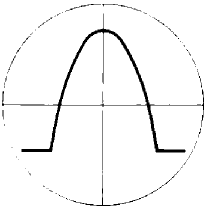
\includegraphics[width=6cm]{graphics/mod.png}
	\caption{Beispielmode. \cite{skript}}
	\label{fig:mod}
\end{figure}
\begin{figure}
	\centering
	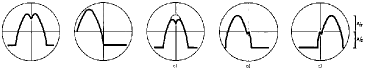
\includegraphics[width=\textwidth]{graphics/mods.png}
	\caption{Einzustellende Moden zur Messung.\cite{skript}}
	\label{fig:mods}
\end{figure}
\subsection{Messung von Wellenlänge, Frequenz und Dämpfung}
Am Ausgang des Klystrons werden eine Messsonde und ein Kurzschluss angebracht. Der Maximalausschlag des SWR Meters liegt jetzt bei ca. $\SI{210}{\volt}$. 

Zur Wellenlängenberechnung wird die Messsonde verschoben, bis sich ein Minimum einstellt. Die Postion der Sonde wird zur weiteren Berechnung notiert. Die Frequenzmessung erfolgt durch Abstimmung des Frequenzmessers auf einen Minimalausschlag des SWR Meters.

Anschließend wird die Frequenz durch Variation der Dämpfung bestimmt. Dazu wird der Kurzschluss durch einen Abschluss ersetzt. Es werden für Dämpfungen im Abstand von $\SI{2}{\deci\bel}$ die Ausschläge notiert.
\subsection{Stehwellenmessung}
Zur Messung der stehenden Wellen wird zusätzlich ein Gleitschraubentransformator in den Hohlleiter eingebaut. Über eine Verschiebung der Messsonde wird ein Minimum eingestellt. Die Einstellungen dafür werden notiert. 

Wenn sich ein Minimum eingestellt hat, wird das SWR Meter auf $\SI{3}{\deci\bel}$ eingestellt. Die Sonde wird bis zu einem Maximum jeweils nach rechts und links verschoben. Die Position wird notiert.

Zum Schluss wird die Wellenlänge mit der Abschwächermethode bestimmt. Die Sondentiefe des Gleitschraubentransformators wird auf $\SI{9}{\milli\meter}$ eingestellt. Bei einer Dämpfung von $\SI{20}{\deci\bel}$ wird das SWR Meter auf eine Ausschlag von $\SI{3}{\deci\bel}$ eingestellt. Mittels Verschiebung der Sonde werden, während mit dem Dämpfungsglied nachgeregelt wird, relative Maxima gesucht. Die Position der Sonde wird notiert.
